% Especificaciones del tamaño de letra, tamaño de hoja, márgenes, librerias, etc.
\documentclass[12pt, letterpaper]{article}
\usepackage[english]{babel}
\usepackage[utf8]{inputenc}
\usepackage[T1]{fontenc}
\usepackage{mathrsfs}
\usepackage{amsmath}
\usepackage{graphicx}
\usepackage{subcaption}
\usepackage{hyperref}
\usepackage{url}
\usepackage{amssymb}
\usepackage{float}
\usepackage[framed, numbered]{matlab-prettifier}
%\usepackage[framed, numbered, autolinebreaks, useliterate]{mcode}
\usepackage[margin=1in]{geometry}
\renewcommand{\baselinestretch}{1.5}

% Enlace Bibliografía
\usepackage{csquotes}
\usepackage[notes,backend=biber]{biblatex-chicago}
\addbibresource{referencias.bib}

% Titulo, autores, fecha.
\title{Práctica \#2: Modelado y Simulación de Sistemas}
\author{Carlos Vásquez 1155057}

% Inicio del documento
\begin{document}
\maketitle

\section*{Introducción}

El modelado de sistemas dinámicos es de gran importancia debido a la información que podemos obtener de estos modelos matemáticos. Por lo regular realizamos estos modelos para mejorar lo que sabemos acerca de un sistema o también puede ser por la necesidad de conocer el comportamiento de una variable que es parte del sistema. Sea cual sea el motivo, es necesario analizarlo de una manera correcta.

A pesar de la gran utilidad que brinda el realizar modelos dinámicos, usualmente resultan ser bastante complicados, siendo éstos expresados en términos de razones de cambio e integrales. Estos inconvenientes pueden evitarse si utilizamos las herramientas matemática adecuadas. En esta práctica nos enfocaremos en el análisis de sistemas dinámicos relativamente sencillos, y sobre todo nos apoyaremos en la transformada de Laplace como herramienta principal para lograr obtener resultados útiles que nos den información acerca de las variables que deseamos medir.

\section*{Desarrollo}

\begin{enumerate}
	\item Construya en SIMULINK el modelo de bloques que resuelva la siguiente ecuación diferencial:
		\begin{equation}
			\frac{dx}{dt} = 3 \sin (2t)
		\end{equation}
		\begin{figure}[H]
			\centering
			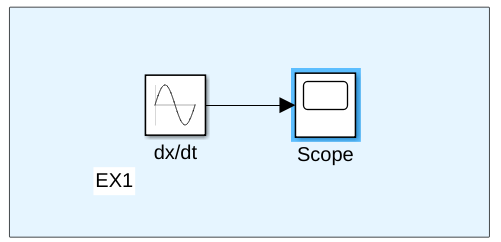
\includegraphics[width=0.5\textwidth]{1.png}
			\caption{Bloques necesarios para el ejercicio 1.}
		\end{figure}

		\begin{figure}[H]
			\centering
			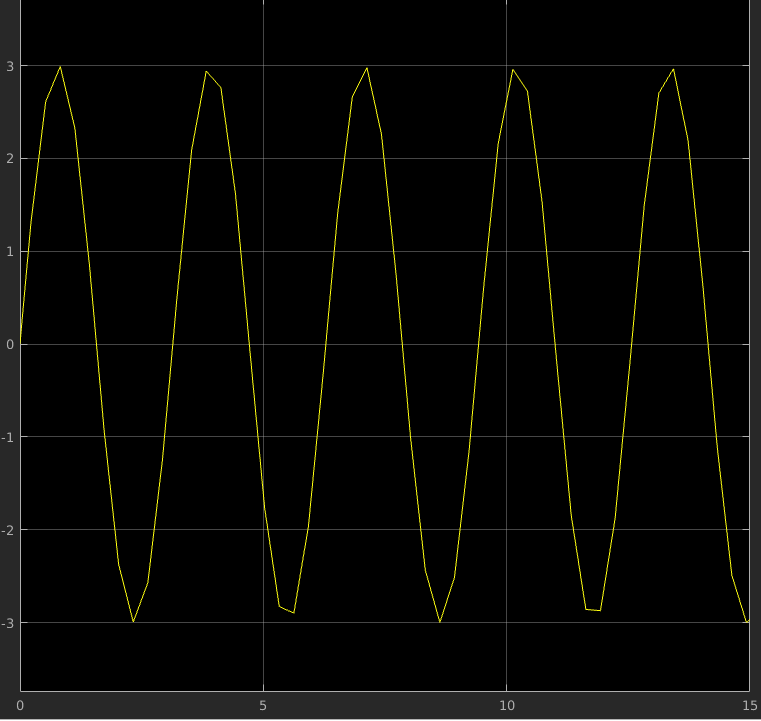
\includegraphics[width=0.5\textwidth]{2.png}
			\caption{Gráfica de la señal de salida.}
		\end{figure}
	\item Sea el siguiente sistema mecánico mostrado en la figura:
		\begin{figure}[H]
			\centering
			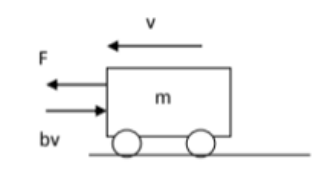
\includegraphics[width=0.4\textwidth]{3.png}
		\end{figure}
		\begin{enumerate}
			\item Defina la ecuación diferencial de primer orden que representa el sistema con salida V.
			\item Genere el modelo en SIMULINK asumiendo los siguientes valores: M = 1000 kg, b = 40 Nm/s. Ajuste el nivel de la fuerza de entrada como un escalón de amplitud de 400 N. Ajuste el tiempo de simulación a 150 s para observar el estado estable.
			\item Cambie la entrada de fuerza por una rampa con un valor de saturación de 200 N.
			\item Encuentre la función de transferencia de acuerdo al modelo obtenido en el inciso (a). Genere el modelo de SIMULINK correspondiente y vuelva a monitorear la salida.
		\end{enumerate}
		Para el inciso (a):
		\begin{equation}
			\boxed{m \frac{dv}{dt} + b v(t) = F(t)}
		\end{equation}
		Para el inciso (b):
		\begin{figure}[H]
			\centering
			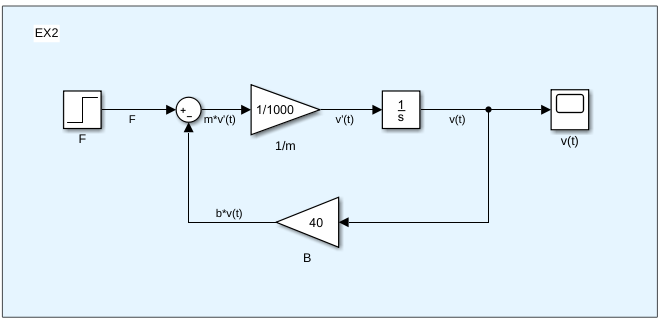
\includegraphics[width=0.8\textwidth]{4.png}
			\caption{Modelo expresado con diagrama de bloques.}
		\end{figure}

		\begin{figure}[H]
			\centering
			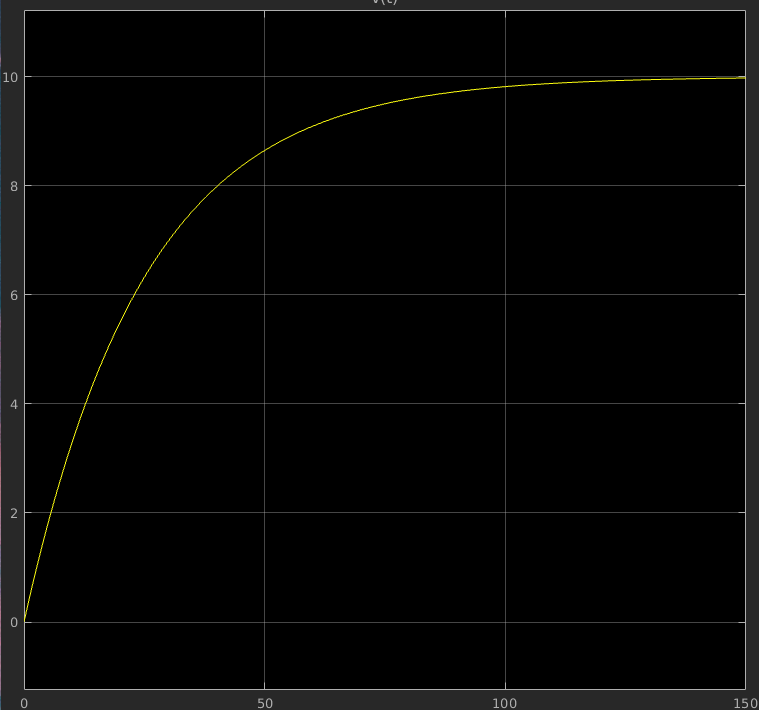
\includegraphics[width=0.5\textwidth]{5.png}
			\caption{Respuesta del sistema.}
		\end{figure}
		Para el inciso (c):
		\begin{figure}[H]
			\centering
			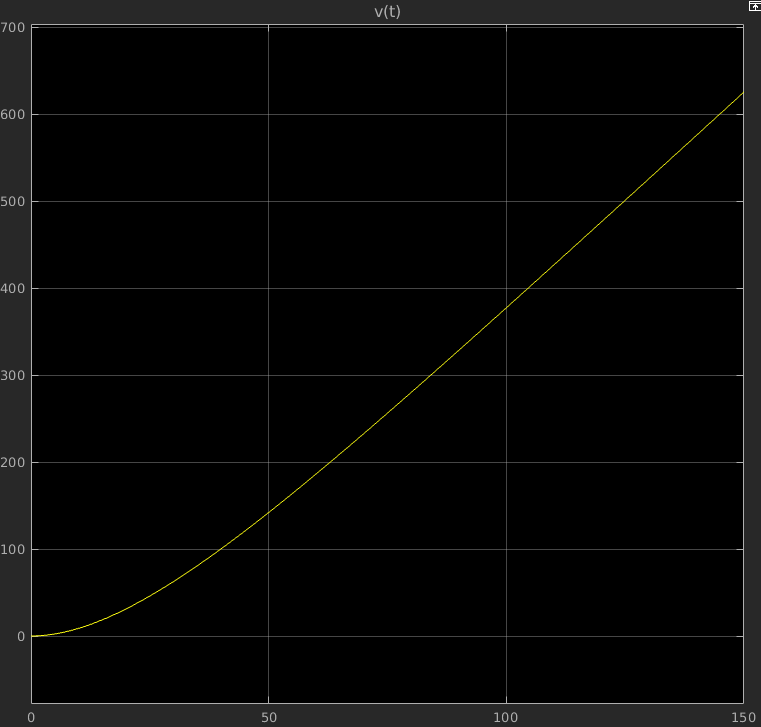
\includegraphics[width=0.5\textwidth]{6.png}
			\caption{t vs. v(t)}
		\end{figure}
		Para el inciso (d):
		Dada la ecuación de (a), podemos aplicar la transformada de Laplace.
		\begin{equation}
			F(s) = MsV(s) + BV(s)
		\end{equation}
		\begin{equation}
			\boxed{\frac{V(s)}{F(s)} = \frac{1}{1000s + 40}}
		\end{equation}

		\begin{figure}[H]
			\centering
			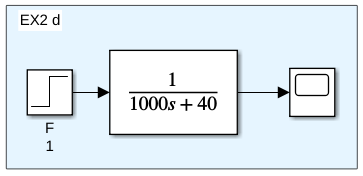
\includegraphics[width=0.5\textwidth]{7.png}
			\caption{Diagrama de bloques de la función de transferencia.}
		\end{figure}

		\begin{figure}[H]
			\centering
			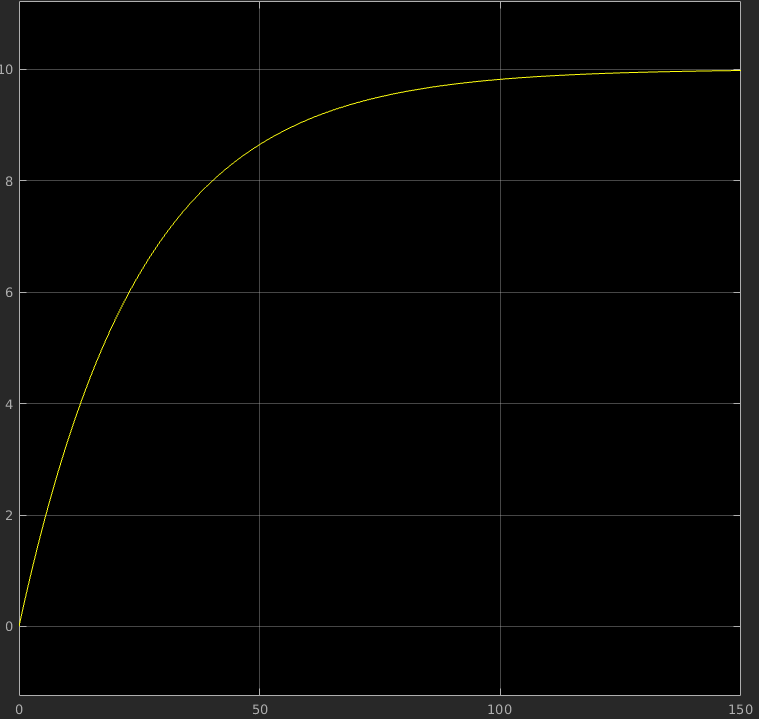
\includegraphics[width=0.5\textwidth]{8.png}
			\caption{Respuesta de la función de transferencia.}
		\end{figure}
	\item Sea el siguiente sistema eléctrico mostrado en la figura.
		\begin{figure}[H]
			\centering
			
\includegraphics[width=0.5\textwidth]{9.png}
		\end{figure}
		\begin{enumerate}
			\item Determinela ecuación diferencial del sistema para una salida Vc.
			\item Genere el modelo en SIMULINK y monitoree el voltaje Vc. Ajuste los calores de R=3, L=1, C=0.5 y la fuente de entrada sea una función escalón de amplitud 2.
			\item Encuentre la función de transferencia de acuerdo al modelo obtenido en el inciso (a). Genere el modelo de SIMULINK correspondiente y vuelva a monitorear la salida.
		\end{enumerate}
		Para el inciso (a):
		\begin{equation}
			v(t) = Ri(t) + L\frac{di(t)}{dt}+ \frac{1}{C} \int i(t) dt
		\end{equation}
		\begin{equation}
			i(t) = C \frac{d v_c(t)}dt{}
		\end{equation}
		\begin{equation}
			\boxed{v(t) = RC\frac{dv_c(t)}{dt} + LC \frac{d^2 v_c(t)}{dt^2} + v_c(t)}
		\end{equation}
		Para el inciso (b):

		\begin{figure}[H]
			\centering
			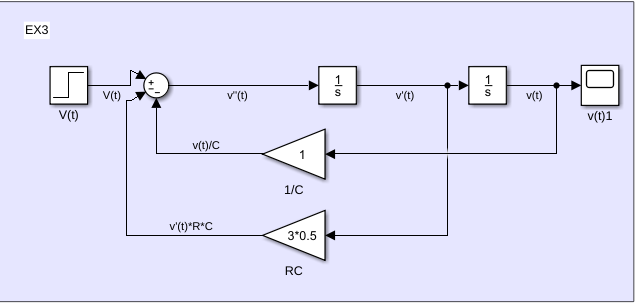
\includegraphics[width=0.7\textwidth]{10.png}
			\caption{Diagrama de bloques para el sistema eléctrico.}
		\end{figure}

		\begin{figure}[H]
			\centering
			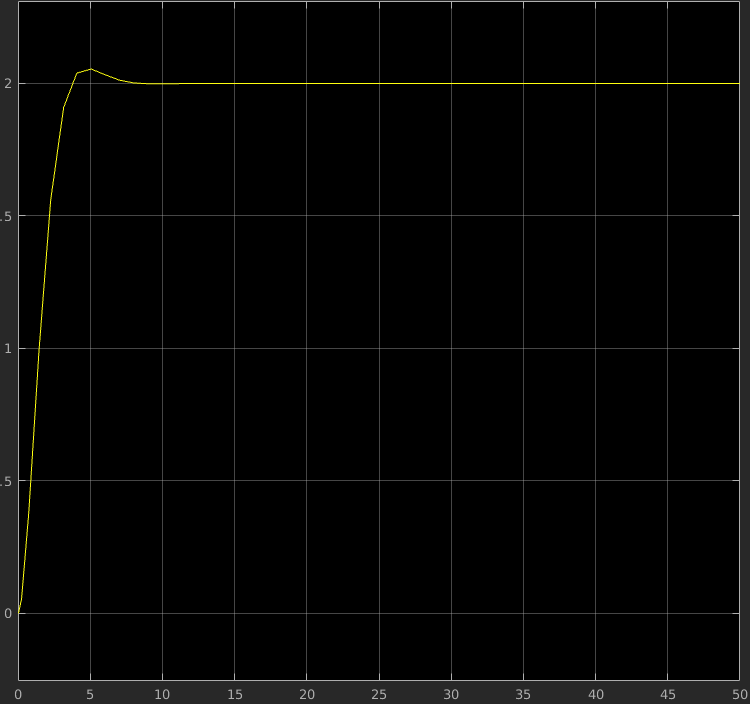
\includegraphics[width=0.5\textwidth]{11.png}
			\caption{Gráfica de la salida.}
		\end{figure}
		Para el inciso (c):
		\begin{equation}
			\frac{V_c(s)}{V(s)} = \frac{1}{LCs^2 + RCs + 1}
		\end{equation}
		\begin{equation}
			\boxed{\frac{V_x(s)}{V(s)} = \frac{1}{s^2 + 1.5s + 1}}
		\end{equation}

		\begin{figure}[H]
			\centering
			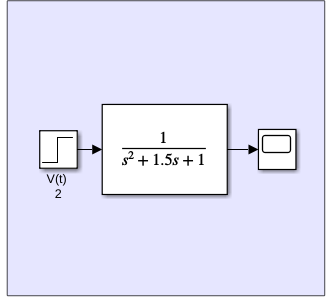
\includegraphics[width=0.5\textwidth]{12.png}
			\caption{Diagrama de bloque, función de transferencia.}
		\end{figure}

		\begin{figure}[H]
			\centering
			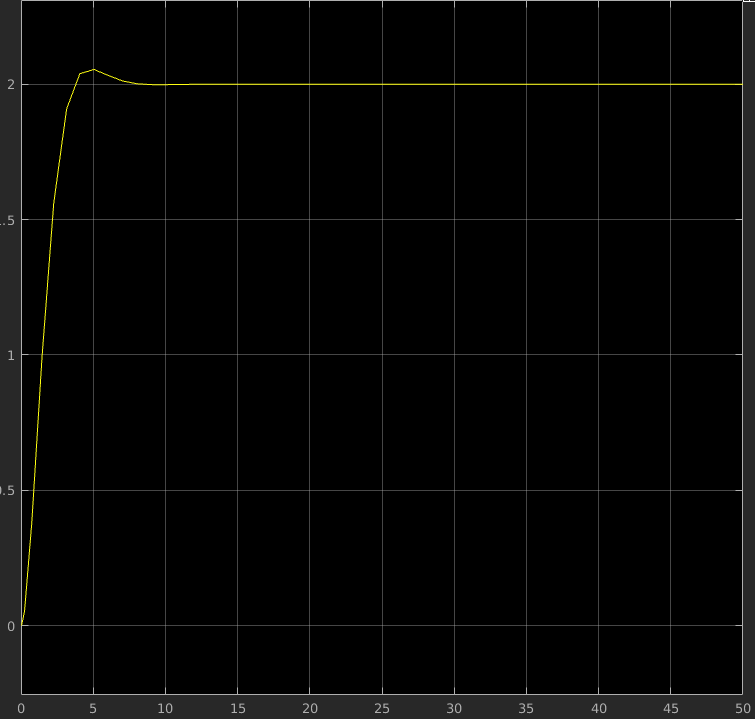
\includegraphics[width=0.5\textwidth]{13.png}
			\caption{Gráfica de la respuesta con la función de transferencia.}
		\end{figure}
	\item Dado el siguiente sistema eléctrico
		\begin{figure}[H]
			\centering
			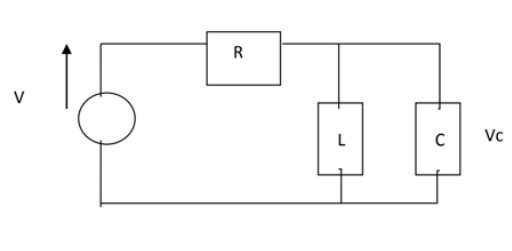
\includegraphics[width=0.5\textwidth]{14.png}
		\end{figure}
		Encuentre la función de transferencia del sistema y genere en SIMULINK el modelo correspondiente. Monitoree la salida para V = 100 @ 60 Hz, R = 500, L = 10 $\mu H$, C = 10 pF.

		\begin{equation}
			v(t) = Ri_1(t) + L \frac{di_1(t)}{dt} - L\frac{di_2(t)}{dt}
		\end{equation}
		\begin{equation}
			0 = -L \frac{di_1(t)}{dt} L \frac{di_2(t)}{dt} + \frac{1}{C} \int i_2(t) dt
		\end{equation}
		\begin{equation}
			V(s) = RI_1(s) + LsI_1(s) - LsI_2(s)
		\end{equation}
		\begin{equation}
			0 = -LsI_1(s) + LsI_2(s) + \frac{1}{Cs}I_2(s)
		\end{equation}
		Sustituyendo y despejando:
		\begin{equation}
			\boxed{\frac{V_c(s)}{V(s)} = \frac{Ls}{RLCs^2 + Ls + R}}
		\end{equation}
		\begin{figure}[H]
			\centering
			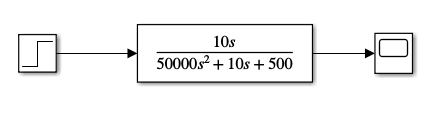
\includegraphics[width=0.5\textwidth]{15.png}
			\caption{Diagrama de bloques para la función de transferencia.}
		\end{figure}

		\begin{figure}[H]
			\centering
			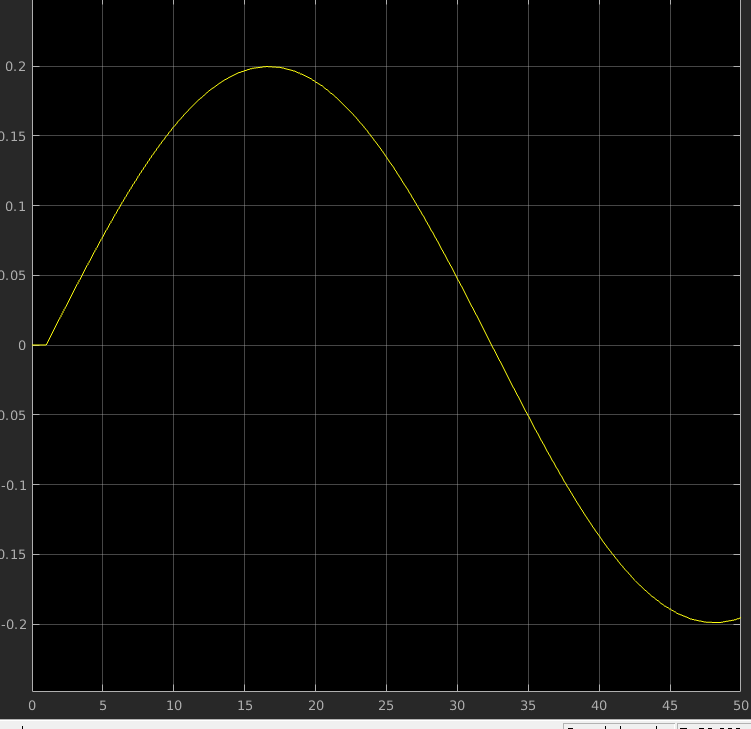
\includegraphics[width=0.5\textwidth]{16.png}
			\caption{Respuesta del sistema.}
		\end{figure}
	\item Obtener modelo matemático y función de transferencia de un motor DC con un movimiento rotacional y acoplado con poleas o coreas. El circuito eléctrico de la armadura y el diagrama del cuerpo libre se muestra a continuación.

		\begin{figure}[H]
			\centering
			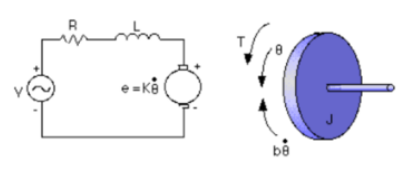
\includegraphics[width=0.5\textwidth]{17.png}
		\end{figure}

		Solución al sistema a partir de las ecuaciones diferenciales ya utilizadas anteriormente:
		\begin{equation}
			v_1(t) = Ri_1(t) + L \frac{di_1(t)}{dt} + e
		\end{equation}
		\begin{equation}
			T(t) = J \frac{d^2 \theta (t)}{dt} + b\frac{d \theta}{dt}
		\end{equation}

		\begin{figure}[H]
			\centering
			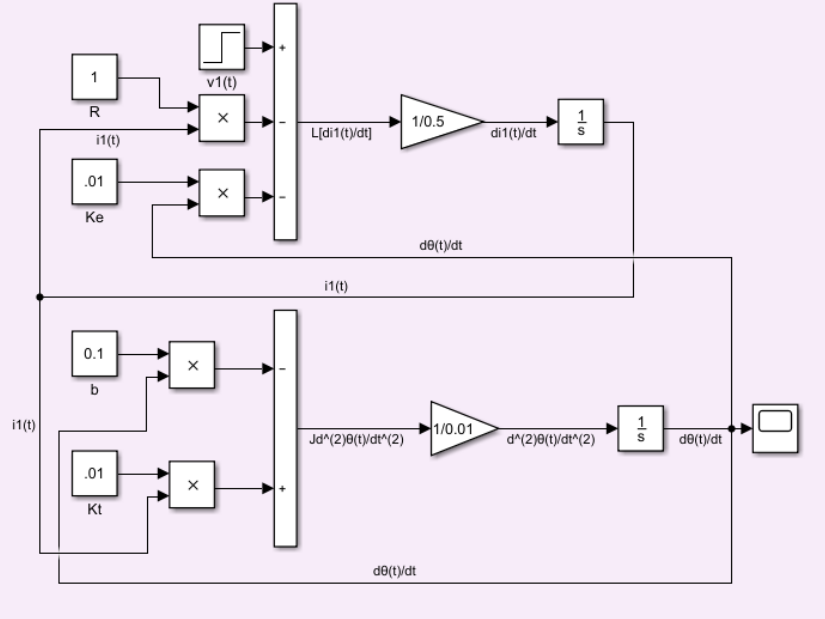
\includegraphics[width=0.5\textwidth]{18.png}
			\caption{Diagrama de bloques del sistema dinámico.}
		\end{figure}

		\begin{figure}[H]
			\centering
			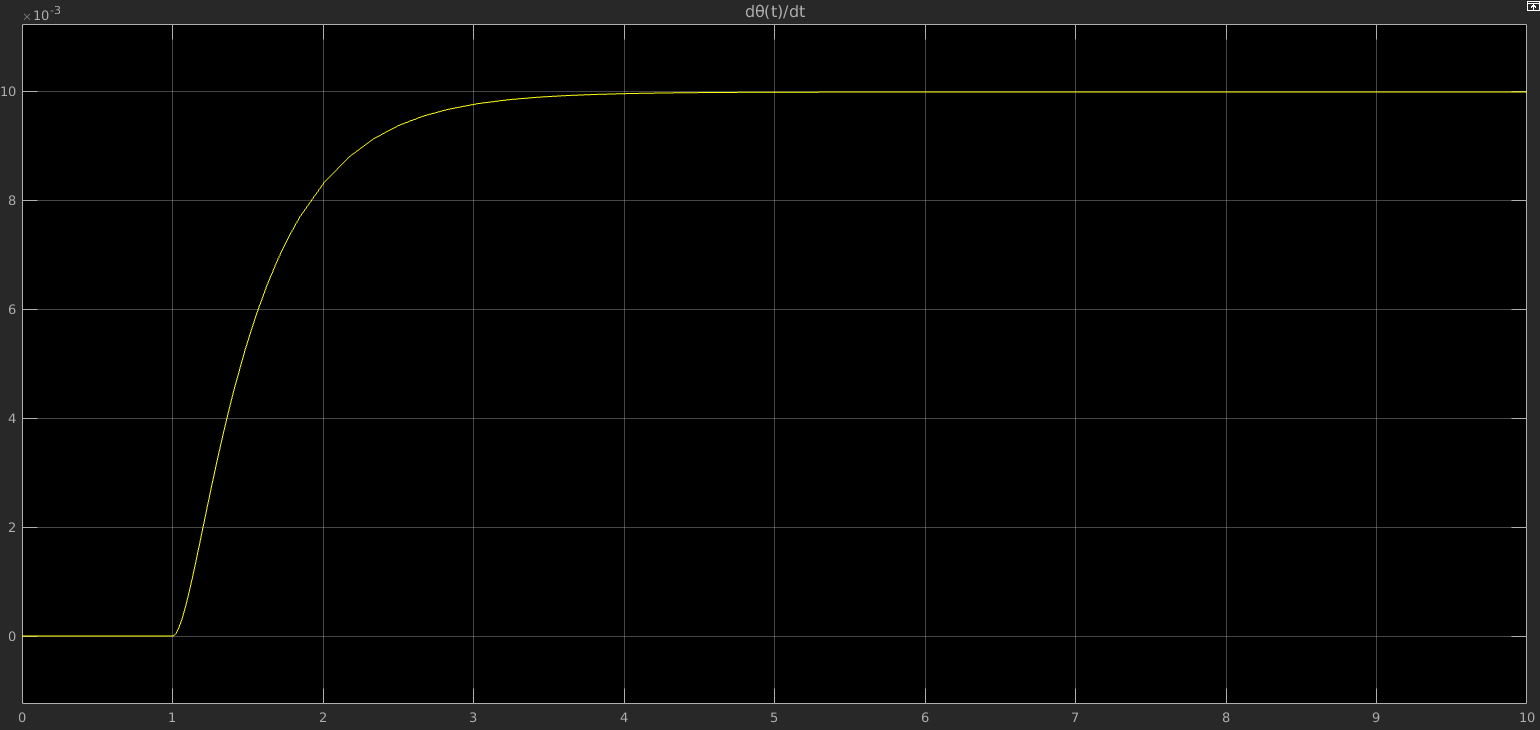
\includegraphics[width=0.9\textwidth]{19.png}
			\caption{Grafica de la variación del torque a lo largo del tiempo.}
		\end{figure}
\end{enumerate}
\section*{Conclusión}
Como hemos observado, analizar estos sistemas mediante ecuaciones diferenciales y transformarlas a ecuaciones algebráicas a través de la transformada de Laplace resulta muy conveniente y algo en lo que podemos apoyarnos para comprender mejor el funcionamiento de estos sistemas. Así podemos obtener información importante de éstos y resolver problemas, diseñar sistemas complejos, entre otras cosas de interés para la ingeniería.
%%%%%  Bib
\renewcommand\refname{Referencias}
\printbibliography
\end{document}
